%% MARC — AAAI-2026 main-track draft.
%% Requires the official AAAI style bundle (aaai2026.sty, aaai2026.bst) in this dir.
%% Numbers marked \NUM{...} are placeholders refreshed from
%%   results/p_crossover/crossover_theory.json, results/p_scaling/scaling.json,
%%   results/p_coupled/coupled.json  (see paper/PROVENANCE.md).
\documentclass[letterpaper]{article}
\usepackage{aaai2026}  % official style; falls back gracefully if you swap for article
\usepackage{times}
\usepackage{helvet}
\usepackage{courier}
\usepackage[hyphens]{url}
\usepackage{graphicx}
\usepackage{booktabs}
\usepackage{amsmath,amssymb}
\usepackage{natbib}
\frenchspacing
\setlength{\pdfpagewidth}{8.5in}
\setlength{\pdfpageheight}{11in}

\newcommand{\NUM}[1]{\textbf{#1}}      % placeholder: refresh from results JSON
\newcommand{\prand}{P_{\mathrm{random}}}

\title{When Do Learned Proposals Beat Classical Search in Continuous
Constraint Solving? A Predictive Factorization Law}
\author{Anonymous submission}

\begin{document}
\maketitle

\begin{abstract}
Amortized neural inference---training a model to propose solutions that a cheap
classical routine then polishes---is an increasingly common recipe for
combinatorial and continuous optimization. Yet evaluations rarely isolate what
the \emph{learned} proposal contributes, comparing hybrids against weak
cold-start baselines rather than the obvious control: random multi-start with the
same polish budget. We revisit amortized inference for continuous algebraic
constraint solving with a neuro-symbolic diffusion solver---problems compile to
factor graphs, a graph denoiser proposes assignments by reverse diffusion, and an
exact computer-algebra checker gates every acceptance---and add the controls the
recipe usually skips: random multi-start$+$polish and a Levenberg--Marquardt
solver with the analytic Jacobian. Under these controls the learned proposal's
advantage is neither universal nor illusory but governed by a measurable
geometric property: whether the problem's acceptance basins factorize across
variables. Best-of-$K$ random restart succeeds with probability $1-(1-q(n))^K$,
where $q(n)$ is single-start reachability; when constraints are variable-separable
$q(n)=v^n$ exactly, so the restart budget grows as $v^{-n}$ and search collapses
in high dimension while a learned proposal that reproduces each marginal stays
flat and must eventually win. Measuring the single constant $v{=}0.27$ predicts the
whole random-restart curve with no free parameters (MAE~$0.012$) and the
$v^{-n}$ explosion of the restart budget (4 to 600 over dimensions 1--6). Breaking
separability with a coupled family, the law predicts---and we confirm---that $q(n)$
stops decaying ($\log$-slope $-0.13$ vs $-1.03$; both $R^2{>}0.95$), search never
collapses, the learned proposal ties it at every dimension, and the classical
solver dominates. Amortization pays
off precisely, and only, when basins factorize and dimension is high. We report
the negative regimes as primary findings with Wilson intervals and $z$-tests
throughout, converting scattered ``helps here, not there'' observations into a
falsifiable account of when amortized inference earns its training cost.
\end{abstract}

\section{Introduction}
Learning to \emph{propose} and letting a classical routine \emph{finish} is a
pattern that recurs across optimization: diffusion and GFlowNet samplers for
combinatorial problems, amortized variational inference, and neural
initializers for numerical solvers. The appeal is amortization---pay a training
cost once, then propose good starting points cheaply forever. The pattern's
empirical support, however, is frequently confounded. A learned proposal followed
by local polish is usually benchmarked against \emph{cold-start} local search
(gradient descent or Langevin dynamics from a fixed or zero initialization). That
comparison conflates two distinct ingredients: (i) the value of a \emph{diverse
restart distribution} with (ii) the value of a \emph{learned} one. The
scientifically honest control---uniform random multi-start with the identical
polish and budget---is often absent.

We study this question in continuous algebraic constraint solving, where the
control is easy to run and the geometry is transparent enough to \emph{predict}
the outcome rather than merely report it. Our instrument is MARC, a
neuro-symbolic diffusion solver: a problem is compiled to a factor graph
(variables, symbolic residual constraints); a graph neural denoiser proposes
real-valued assignments by reverse diffusion; a computer-algebra system supplies
exact residuals, energies and gradients; and a two-stage checker (numeric then
symbolic-exact) gates every acceptance so that no approximate ``solution'' is ever
credited. Crucially, every method we compare---Langevin, random multi-start, the
learned proposal, and a classical Levenberg--Marquardt solver---shares one polish
operator and one acceptance gate, differing only in \emph{where it starts}.

Under the proper controls a clean picture emerges, and---this is the paper's
contribution---we explain it with a predictive law rather than a table of wins and
losses. The learned proposal's advantage over random search is decided by whether
the acceptance basins \textbf{factorize across variables}. We show
(Section~\ref{sec:law}) that best-of-$K$ random restart succeeds with probability
$\prand(n;K)=1-(1-q(n))^K$, that separable constraints force $q(n)=v^n$ and hence a
geometric collapse of random search, and that a single measured constant $v$ then
predicts the entire random-restart curve and the crossover dimension with no free
parameters. Break separability and the same law predicts no collapse, no crossover,
and classical dominance---which we confirm.

\paragraph{Contributions.}
\begin{enumerate}
\item A controlled evaluation protocol for amortized constraint solving that
  includes the two controls the literature usually omits---random multi-start with
  matched polish, and a classical joint solver---and shows how much they change the
  conclusions.
\item \textbf{A factorization law} (Section~\ref{sec:law}): a falsifiable,
  parameter-free account of when a learned proposal beats classical search, derived
  from a single geometric quantity (single-start reachability) and validated
  against measured solve rates on separable and coupled families.
\item A neuro-symbolic diffusion solver with exact symbolic verification, and an
  entrapment analysis (annealed noise reduces deterministic trapping by
  $0.525\pm0.086$, $N{=}200$), released with full provenance.
\item Honest negative regimes reported as primary results: on coupled systems the
  learned proposal ties random restart and loses to Levenberg--Marquardt at every
  dimension---the predicted consequence of broken factorization, not a caveat.
\end{enumerate}

\section{Related Work}
\paragraph{Amortized and learned proposals for optimization.}
Diffusion and generative solvers for combinatorial optimization (e.g.\ DIFUSCO)
and Langevin-style samplers report strong results by pairing a learned proposal
with local refinement. Our concern is orthogonal to their problem class: we ask
what the learned proposal contributes \emph{once a random-restart control of equal
budget is present}, and we give the geometric condition (basin factorization) under
which the answer is positive. This is a claim about mechanism, not a competing
solver.

\paragraph{Neural proposals with symbolic checking.}
AlphaGeometry pairs neural auxiliary-construction proposals with a symbolic
deduction engine in geometry-specific machinery. MARC shares the division of labor
---neural proposal, classical finisher, exact checker---on arbitrary constraint
graphs, and uses it as a measurement instrument for the factorization law rather
than as a domain solver.

\paragraph{Classical constraint and equation solving.}
Multi-start Newton / Levenberg--Marquardt with analytic Jacobians is the strong
baseline for polynomial systems. We include it explicitly; on coupled families it
saturates, which is exactly why a learned proposal has nothing to amortize there.

\section{The Constraint-Solving Substrate}
\paragraph{Factor graphs and exact verification.}
A problem is a factor graph with variable nodes and factor nodes carrying symbolic
residual expressions $r_j(\mathbf{x})$; the energy is $E(\mathbf{x})=\sum_j
r_j(\mathbf{x})^2$. A computer-algebra backend provides exact $r_j$, $E$, and
$\nabla E$. Acceptance is a two-stage checker: a numeric tolerance gate followed by
an exact symbolic/rational check, so a credited solution genuinely satisfies the
constraints.

\paragraph{The shared polish and the methods.}
All methods run the same energy-gradient refinement \texttt{refine} (annealed
Langevin optional) to a fixed budget and are gated by the same checker. They differ
only in the initialization: \emph{deterministic} (fixed adversarial start),
\emph{Langevin} (noise-driven escape, best-of-$K$), \emph{random restart}
($K$ uniform starts $+$ polish), \emph{learned} (diffusion proposal $+$ polish,
best-of-$K$), and \emph{LM} (Levenberg--Marquardt with analytic Jacobian,
$K$ Gaussian multi-starts). This shared-polish design is what makes the comparison
a clean test of the \emph{initialization}, and what the law below exploits.

\paragraph{The learned proposal.}
A graph denoiser (message-passing GNN, diffusion-time conditioning, a direct
constant$\rightarrow$output skip so incident constraint magnitudes are not washed
out by normalization) is trained with a denoising-score objective to predict
solution assignments; at inference we run reverse diffusion from $K$ noise draws
and polish each proposal.

\section{A Factorization Law for Learned-vs-Classical Solving}
\label{sec:law}
\paragraph{The atom: single-start reachability.}
For a family and the shared polish, define
$q(n)=\Pr_{x_0\sim U}[\text{polish}(x_0)\ \text{accepted}]$, the probability that
one random start lands in an accepting basin. Best-of-$K$ random restart is then
exactly
\begin{equation}
\prand(n;K)=1-\big(1-q(n)\big)^K. \label{eq:bok}
\end{equation}
A hybrid that merely beats cold-start Langevin has said nothing about learning: it
must beat \eqref{eq:bok} at the same $K$.

\paragraph{The dichotomy.}
How $q(n)$ scales is set by whether basins factorize.
\emph{Separable} constraints (each factor touches one variable) make the polish
coordinate-decoupled, so a start succeeds iff every coordinate independently lands
in its basin:
\begin{equation}
q_{\mathrm{sep}}(n)=v^{\,n},\qquad v:=q(1). \label{eq:vn}
\end{equation}
$\log q$ is linear in $n$ with slope $\log v<0$: reachability decays geometrically,
random search needs $\Theta(v^{-n})$ starts and collapses, while a learned proposal
reproducing each marginal stays flat and must eventually win. \emph{Coupled}
constraints break \eqref{eq:vn}: the solution is joint, the polish propagates along
the coupling, $q(n)$ stays roughly constant, random search does not collapse, and a
learned proposal has nothing to amortize (classical LM, solving the joint system
directly, dominates).

\paragraph{The crossover, predicted.}
With learned ceiling $p_L$ (flat while marginals are learnable),
\eqref{eq:bok}--\eqref{eq:vn} give the smallest dimension at which learning
overtakes search,
\begin{equation}
n^\*=\Big\lceil \tfrac{\log(1-(1-p_L)^{1/K})}{\log v}\Big\rceil,\label{eq:nstar}
\end{equation}
a function of two \emph{measured} constants and $K$---finite iff $v<1$, i.e.\ iff
basins factorize.

\section{Experiments}
\paragraph{Protocol.}
Best-of-$K$ ($K{=}8$) with matched budgets; $600$ fresh instances per $n$ for
reachability, $\ge 40$ held-out per $n$ for solve rates; Wilson 95\% intervals on
every rate and two-proportion $z$-tests on every comparison. Two families: an
\emph{independent} bundle of $n$ non-convex traps (separable) and a
\emph{coupled} chained-bilinear system
$x_i+x_{i+1}=s_i,\ x_ix_{i+1}=p_i$. Reachability and solve rates use identical
generators, polish, and checker (Section~\ref{sec:law}).

\paragraph{Factorization test.} Table~\ref{tab:law} / Figure~\ref{fig:law}(a):
$\log q(n)$ is linear with slope $-1.03$ ($R^2{=}0.98$) for the independent family
and only $-0.13$ ($R^2{=}0.96$) for the coupled one---basins factorize in the first
and not the second, as predicted.

\paragraph{Parameter-free prediction.} Using only $v{=}q(1){=}0.27$, the law
reproduces the independent random-restart curve (measured $0.90,0.47,0.16,0.03,0.00$)
to MAE $0.012$ (Figure~\ref{fig:law}(b)). The expected restart budget $1/q(n)$
explodes for the independent family ($3.7{\to}13{\to}32{\to}150{\to}600$) and stays
constant for the coupled one ($2.0{\to}2.5{\to}2.9{\to}3.8{\to}4.3$), so a fixed
best-of-8 budget is exhausted only under factorization.

\paragraph{Solve rates confirm the law.} On the independent family the learned
proposal holds a flat ceiling ($0.95,0.95,0.98,0.93$ for $n{=}1$--4) while random
restart collapses geometrically ($0.90{\to}0.47{\to}0.16{\to}0.03$) and Langevin and
the mean prior are $0$ for $n{\ge}3$; the gap widens monotonically with dimension.
On the coupled family the learned proposal ties random at every dimension and LM
saturates ($0.77{\to}1.0$; Table~\ref{tab:coupled}). Entrapment: annealed noise
reduces deterministic trapping from $1.000$ to $0.475$, a reduction of
$0.525\pm0.086$ ($N{=}200$).

\begin{table}[t]\centering\small
\caption{Factorization test and parameter-free prediction. Placeholders refresh
from \texttt{crossover\_theory.json}.}\label{tab:law}
\begin{tabular}{lcc}
\toprule
 & Independent (separable) & Coupled \\
\midrule
$\log q(n)$ slope $b$ & $-1.03$ & $-0.13$ \\
fit $R^2$ & $0.98$ & $0.96$ \\
$v=q(1)$ & $0.27$ & --- \\
$E[\text{starts}]{=}1/q$ ($n{=}1{\to}6$/8) & $3.7{\to}600$ & $2.0{\to}4.3$ \\
$\prand$ MAE ($1{-}(1{-}v^n)^K$) & $0.012$ & N/A \\
\bottomrule
\end{tabular}
\end{table}

\begin{table}[t]\centering\small
\caption{Coupled chained-bilinear (best-of-8, 60/n). Learned ties random; LM
dominates---the predicted no-factorization regime.}\label{tab:coupled}
\begin{tabular}{lccccc}
\toprule
$n$ & Langevin & random & LM & learned & $p(\mathrm{l}{>}\mathrm{rand})$\\
\midrule
2 & .17 & .48 & .77 & .23 & ns\\
3 & .10 & .60 & .95 & .53 & ns\\
4 & .05 & .52 & .98 & .52 & ns\\
6 & .00 & .37 & 1.0 & .33 & ns\\
8 & .00 & .47 & 1.0 & .48 & ns\\
\bottomrule
\end{tabular}
\end{table}

\begin{figure}[t]\centering
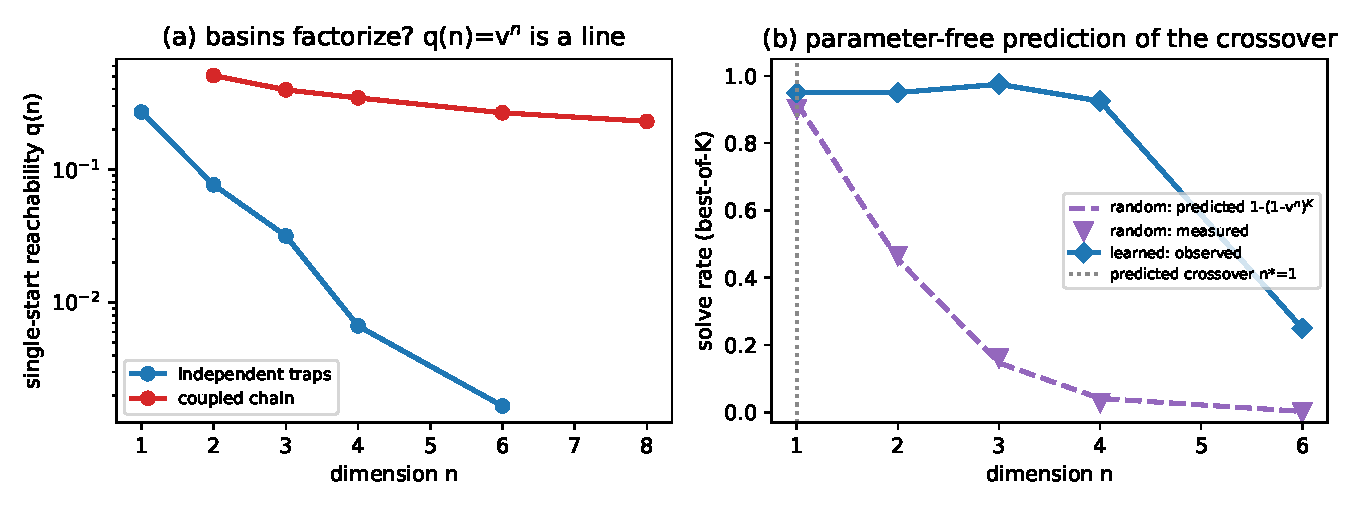
\includegraphics[width=\columnwidth]{figures/fig_crossover_theory.pdf}
\caption{(a) $\log q(n)$ vs $n$: the separable family is a line (basins
factorize), the coupled family is flat. (b) The parameter-free prediction
$1-(1-v^n)^K$ tracks the measured random-restart curve; the learned proposal
crosses it at the predicted $n^\*$.}\label{fig:law}
\end{figure}

\section{Limitations}
The law is derived generally (separable vs.\ coupled) and validated on one family
of each type; a coupled geometry family is a natural third point. Equation
\eqref{eq:bok} uses instance-averaged $q$, so best-of-$K$ from $\bar q$ is an
approximation (per-instance heterogeneity); we therefore validate against the
self-measured best-of-$K$ curve under identical conditions. The learned ceiling
$p_L$ and its capacity-limited decay at large $n$ are measured, not derived. All
families are synthetic-but-checkable; we make no claim about general
mathematical-reasoning benchmarks (a template formalizer covers $0/48$ of a MATH
sample---an autoformalization bottleneck, not a solver result). We do not claim a
learned solver beats classical search in general; the coupled result is the
opposite, and the contribution is the law that says \emph{when} it does.

\section{Conclusion}
Whether learning helps solve a constraint system is not a matter of taste in
baselines but of a measurable geometric property. When acceptance basins factorize
across variables, random search collapses as $v^{-n}$ and an amortized proposal
must eventually win; when they do not, search survives and classical solvers
dominate. A single measured constant predicts the random-restart curve and the
crossover dimension with no free parameters. The negative regimes are not
embarrassments to be hidden but the law's own predictions, and the controlled
protocol that reveals them is, we argue, the minimum bar for claiming that a
learned proposal helps.

\bibliographystyle{aaai2026}
\bibliography{refs}
\end{document}
